\documentclass{article}
\usepackage{graphicx} % Required for inserting images
\usepackage{amsmath}
\usepackage[margin=.5in]{geometry}
\usepackage{float}
\setlength{\parindent}{0pt}

\title{Homework 8}
\author{Quan Nguyen}
\date{April 2026}

\begin{document}
\maketitle
The code for this homework can be found at https://github.com/nguyencquan/Markov2026.
\section{Cycle}

\textbf{a)} The rate matrix is given by the matrix below 

\[
\begin{vmatrix}
    -1&1&0&0\\
    0&-1&1&0\\
    0&0&-1&1\\
    1&0&0&-1\\
\end{vmatrix}
\]

Now to solve the eigenvalue through the use of R eigen function:
\[
\begin{cases}
    \lambda_1 = -2\\
    \lambda_2 = -1+i\\
    \lambda_3 = -1-i\\
    \lambda_4 = 0\\
\end{cases}
\]

\textbf{b)} Find the stationary distribution by using the fact that $Q^T\vec{\pi} = 0$
\[
Q^T = \begin{vmatrix}
    -1&0&0&1\\
    1&-1&0&0\\
    0&1&-1&0\\
    0&0&1&-1\\
\end{vmatrix}
\]
Which then leads to
\[
\begin{vmatrix}
    -1&0&0&1\\
    1&-1&0&0\\
    0&1&-1&0\\
    0&0&1&-1\\
\end{vmatrix}
\begin{vmatrix}
    \pi_1\\
    \pi_2\\
    \pi_3\\
    \pi_4\\
\end{vmatrix} = 0
\]
And since I can use software to solve, using R. I set the first row to 1 in order to normalize
and get a resulting stationary distribution of $\vec\pi = [.25,.25,.25,.25]^T$.

\textbf{c)} We want to know how the convergence to each point occurs. Based on the eigenvalues,
we would solve the differential equation in different ways. Given the master equation:
\[\vec{y'}(t) = Q^T\vec{y}(t)\]
We would get the following solution (eigenvector solved in R):
\[
y(t) = c_1\begin{vmatrix} .5 \\ -.5 \\ .5 \\ -.5 \end{vmatrix} e^{-2t} +
    c_2e^{-t}\left(\begin{vmatrix}.5 \\0 \\ -.5\\0\end{vmatrix}\cos(-t) - \begin{vmatrix}0 \\.5 \\ 0\\-.5\end{vmatrix}\sin(-t)\right)  +
    c_3e^{-t}\left(\begin{vmatrix}.5 \\0 \\ -.5\\0\end{vmatrix}\sin(-t) + \begin{vmatrix}0 \\.5 \\ 0\\-.5\end{vmatrix}\cos(-t)\right) +
    c_4\begin{vmatrix} .5\\.5\\.5\\.5\end{vmatrix}
\]
Based on this equation, we can see that it oscilates due to the sin and cosine but the exponential terms
imply that it exponentially decays overtime too. This means that there is a dampened oscilation over time until
it eventually converges to a stationary distribution of $[.25,.25,.25,.25]^T$. (Note that
$\lim_{t\to \infty}y(t) = \pi \implies c_4 = .5$). Though on a second round of looking at this, by simply
having a complex eigenvalue, it will have a dampened oscilatory convergence. If it is only real solutions,
then the convergence is exponential.

\textbf{d)} Utilizing the solution that I came up above, we know the value for $c_4$ and we
also set $y(0) = [1/3,2/3,0,0]^T$ and solve for the system of equation (which was also computed in R).

\[
\begin{vmatrix}1/3 \\2/3 \\ 0\\0\end{vmatrix} = 
    c_1\begin{vmatrix} .5 \\ -.5 \\ .5 \\ -.5 \end{vmatrix} +
    c_2\begin{vmatrix}.5 \\0 \\ -.5\\0\end{vmatrix} +
    c_3\begin{vmatrix}0 \\.5 \\ 0\\-.5\end{vmatrix} +
    c_4\begin{vmatrix} .25\\.25\\.25\\.25\end{vmatrix}
\]

\[
\begin{vmatrix}1/3 \\2/3 \\ 0\\0\end{vmatrix} = 
    \begin{vmatrix}
        .5 & .5 & 0 &.25\\
        -.5 & 0 & .5&.25\\
        .5 & -.5 & 0&.25\\
        -.5 & 0 & -.5&.25
    \end{vmatrix}\begin{vmatrix}
        c_1\\c_2\\c_3\\c_4
    \end{vmatrix}
\]
Yielding $c = [-1/6,1/3,2/3,1]^T$, hence the full equation becomes:
\[
y(t) = -\frac{1}{6}\begin{vmatrix} .5 \\ -.5 \\ .5 \\ -.5 \end{vmatrix} e^{-2t} +
    \frac13e^{-t}\left(\begin{vmatrix}.5 \\0 \\ -.5\\0\end{vmatrix}\cos(-t) - \begin{vmatrix}0 \\.5 \\ 0\\-.5\end{vmatrix}\sin(-t)\right)  +
    \frac23e^{-t}\left(\begin{vmatrix}.5 \\0 \\ -.5\\0\end{vmatrix}\sin(-t) + \begin{vmatrix}0 \\.5 \\ 0\\-.5\end{vmatrix}\cos(-t)\right) +
    \begin{vmatrix} .25\\.25\\.25\\.25\end{vmatrix}
\]

\textbf{e)}

We want the equation for the probability of being in state 1 as a function of time
hence we only look at the first index of the vector yielding:
\[
y_1(t) = \frac{-e^{-2t}+e^{-t}(2\cos(t)-4\sin(t))}{12}+.25
\]
\begin{figure}[H]
    \centering
    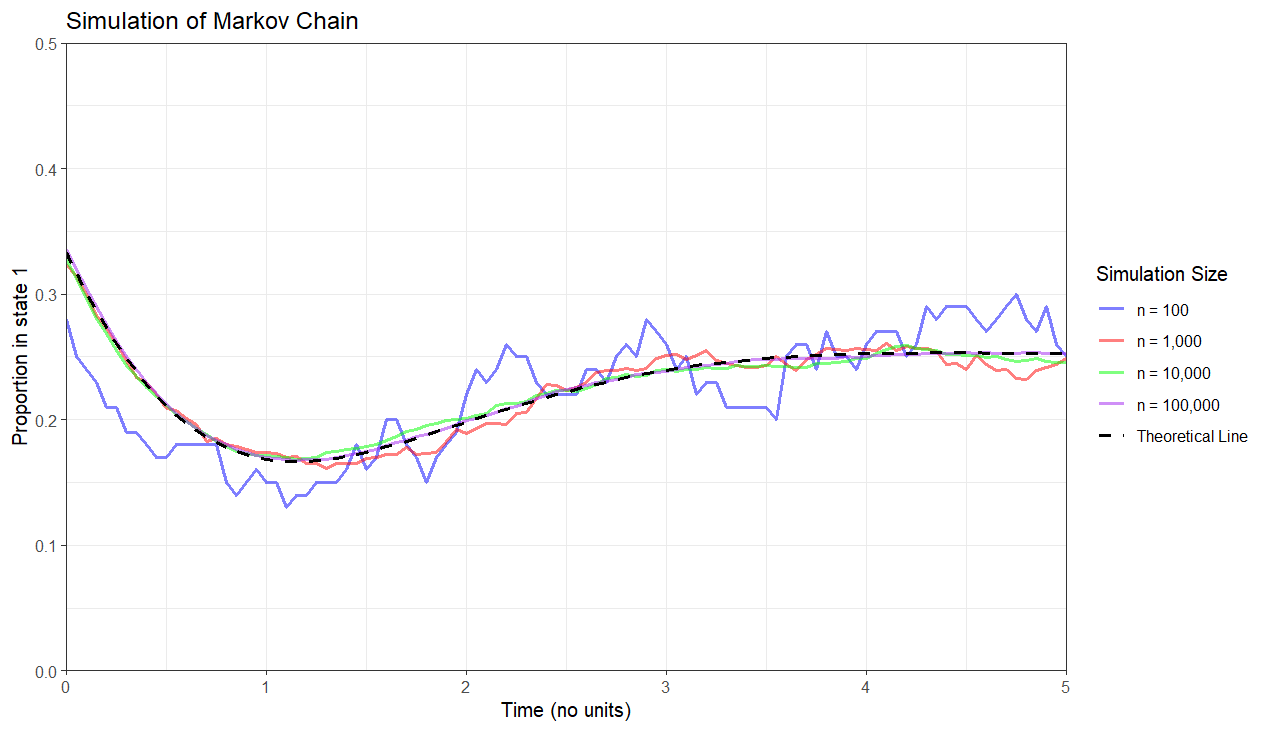
\includegraphics[width=0.7\linewidth]{Simulation.png}
    \caption{Simulation Result of the Markov Chain}
\end{figure}
\section{Receptor Binding}

\textbf{a)} The markov chain was drawn in google drawing.
\begin{figure}[H]
    \centering
    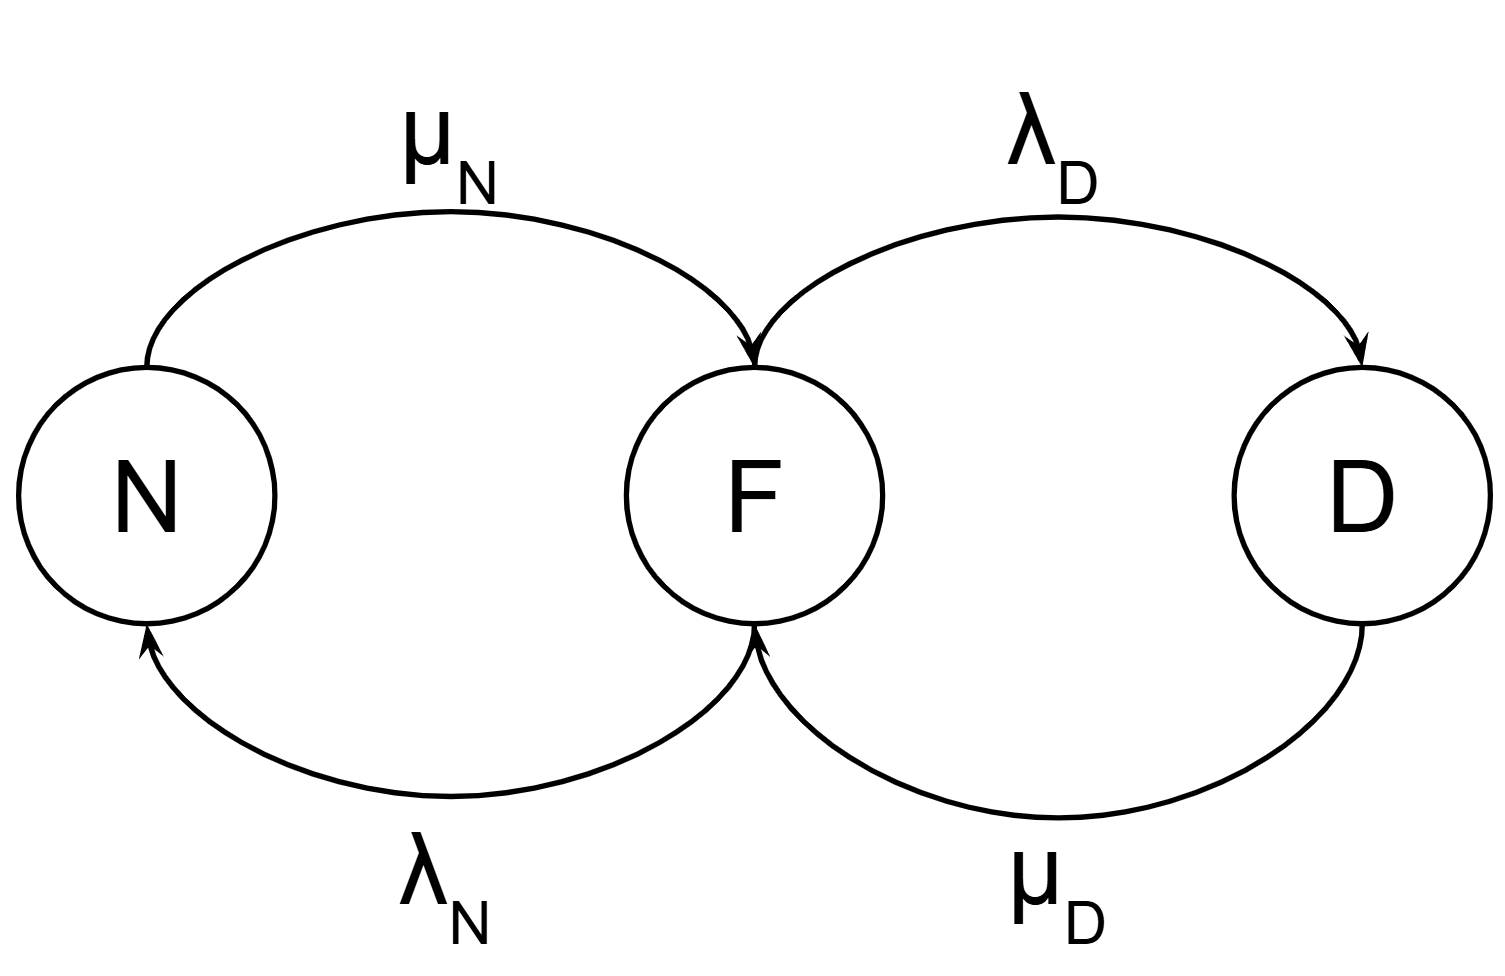
\includegraphics[width=0.7\linewidth]{Markov Chain.png}
    \caption{Markov Chain of Receptor Binding}
\end{figure}

We will be using the following order for subsequent matrices with the Q matrix
being defined as:


\[
Q = \begin{array}{|c c c|}
N & F & D\\
\hline
-\mu_N&\mu_N&0\\
\lambda_N&-(\lambda_N+\lambda_D)&\lambda_D\\
0&\mu_D&-\mu_D\\

\end{array}
\]

\textbf{b)} To solve for the stationary distribution, we must solve for the equation $Q^T\pi = 0$
and substitute $\rho_D=\lambda_D/\mu_D,\rho_N = \lambda_N/\mu_N$

\begin{align*}
    0 &= \begin{vmatrix}
    -\mu_N & \lambda_N & 0\\
    \mu_N & -(\lambda_n + \lambda_D) & \mu_D\\
    0 & \lambda_D & - \mu_D
\end{vmatrix}\begin{vmatrix}
    N \\ F \\ D
\end{vmatrix}\\
&\implies\begin{cases}
    -N\mu_N + F\lambda_N = 0\\
    N\mu_N  -F(\lambda_n + \lambda_D) + D\mu_D=0\\
    F\lambda_D  - D\mu_D=0
\end{cases}\\
&\implies\begin{cases}
    N=F\rho_N\\
    F = \frac{N\mu_N + D\mu_D}{\lambda_N + \lambda_D}\\
    D = F\rho_D
\end{cases}\\
&\implies\begin{cases}
    N=F\rho_N\\
    F = F\frac{\lambda_N + \lambda_D}{\lambda_N + \lambda_D}\\
    D = F\rho_D
\end{cases}\\
&\implies\begin{cases}
    N=F\rho_N\\
    F = F\\
    D = F\rho_D
\end{cases}
\end{align*}
We must keep in mind however that $N+F+D = 1$ as this is the stationary distribution. Hence we set F as 1, and we get
the final normalized distribution of \[\pi = \left[\frac{\rho_N}{1 + \rho_N + \rho_D},\frac{1}{1 + \rho_N + \rho_D},\frac{\rho_D}{1 + \rho_N + \rho_D}\right]^T\]

Let us assume the following cases, and the resultiing distributions:

\[
\begin{cases}
    \rho_N = 0 & \pi = \left[0,\frac{1}{1 + \rho_D},\frac{\rho_D}{1 + \rho_D}\right]^T\\
    \rho_D = 0 &\pi = \left[\frac{\rho_N}{1 + \rho_N},\frac{1}{1 + \rho_N},0\right]^T\\
    \rho_N,\rho_D = 0 &\pi = \left[0,1,0\right]^T\\
    \rho_N \to \infty &\pi = \left[1,0,0\right]^T\\
    \rho_D \to \infty &\pi = \left[0,0,1\right]^T\\
    \rho_N,\rho_D \to \infty &\pi = \left[.5,0,.5\right]^T\\
\end{cases}
\]
When $\rho_X=0$ the molecule X almost never binds to the receptor. On the other hand
if $\rho_X \to \infty$ then molecule X exclusively binds to the receptor. If both rho are 0, then there is no
molecule binding, however if both X approaches infinity (we are assuming the same infinity) then there is an equal 
probability of the receptor being bound by either molecule at any point of time. Though it should be noted that in 
the infinite scenerio, the different binded states are essentially an abosrbing state.

\textbf{c)}
Using the given values we end up with the Q matrix that we will transpose to solve $y'(t) = Q^Ty(t)$:

\[
Q = \begin{array}{|c c c|}
N & F & D\\
\hline
-1&1&0\\
1&-2&1\\
0&1&-1\\
\end{array}
\]

\[
Q^T = \begin{vmatrix}
    -1 & 1 & 0\\
    1 & -2 & 1\\
    0 & 1 & -1
\end{vmatrix}
\]
Solving for the corresponding eigenvalue and rescaling the eigenvectors using R we get:
\[
\begin{cases}
    \lambda_1 = 0 & [1,1,1]^T\\
    \lambda_2 = -1 & [-1,0,1]^T\\
    \lambda_3 = -3 & [-1,2,-1]^T\\
\end{cases}
\]
Hence we end up with the solution:
\[
y(t) = c_1[1,1,1]^T + c_2e^{-t}[-1,0,1]^T + c_3e^{-3t}[-1,2,-1]^T
\]
Given the initial condition of $X_0 = N$ we solve the system of equation using R. Note I substituted
in 1/3 and forced $c_1$ to equal 1 as this accounts for the stationary distribution since
$\lim_{t\to \infty}y(t) = \pi \implies c_1 = 1/3$
\[
[1,0,0]^T = \begin{vmatrix}
    1/3 & -1 & -1\\
    1/3 & 0 & 2\\
    1/3 & 1 & -1
\end{vmatrix}\begin{vmatrix}
    c_1\\ c_2\\c_3
\end{vmatrix} \implies c_1 = 1, c_2 = -1/2, c_3 = -1/6
\]

Substituting in these values and looking at only the 2nd row will yiled when the receptor is open
as the function:
\[
y_F(t) = \frac{1-e^{-3t}}{3}
\]

\section{Ice Cream Waiting}
\textbf{a)}

We are going to be using a Markov Process $\{X(t)\}$ with a state space of $n \geq 0$.
We also know that people will join the line at a rate of 30 an hour which can be modeled by
$q(n,n+1) = 30,\forall n$. Additionally we know people are served at an exponential rate of
1 a minute which will have a rate of 60 per hour. Also each person has a probability of leaving
a queue while not getting ice cream at a rate of 5 an hour. Combining these two and noting
one person getting ice cream we get
$q(n,n-1) = 60 + 5(n-1),n>0$. To create a rate matrix, we have the terms for indexes 
$[n,n+1] = 30$, $[n,n-1] = 60 + 5(n-1)$, $[n,n] = -(90 + 5(n-1))$

\textbf{b)}

Since we know exactly what terms each row must have, we can utilize detailed balancing to solve the 
staitonary distribution with the following abbreviation for simplification:
\[Q^T\pi = 0\]
The following terms will be used for temporary simplification:
\begin{gather*}
\lambda = 30\\ \mu_n = 60 + 5(n-1),\forall n>0\text{ o/w } =0
\end{gather*}
Hence we get the resulting form:

\begin{align*}
    \pi_0\lambda = \pi_1\mu_1\\
    \implies\pi_1 = \frac{\pi_0\lambda}{\mu_1}\\
    \pi_1\lambda = \pi_2\mu_2\\
    \implies \pi_2 = \frac{\pi_0\lambda^2}{\mu_1\mu_2}\\
    \pi_2\lambda = \pi_3\mu_3\\
    \implies \pi_3 = \frac{\pi_0\lambda^3}{\mu_1\mu_2\mu_3}\\
    \implies \pi_n = \pi_0\prod_{i=1}^n \frac{\lambda}{\mu_i}
\end{align*}
Plugging in the terms and solving:
\begin{align*}
    \pi_n &= \pi_0\prod_{i=1}^n \frac{30}{60 +5(i-1)}\\
    &= \pi_0\prod_{i=1}^n \frac{6}{11+i}\\
    &= \frac{\pi_06^n11!}{(n+11)!}
\end{align*}
Note that the above equation also works for $n=0$ to define $\pi_0$

Additionally we must also satisfy the following equation.
\[
\pi_0\sum_{n=0}^\infty \frac{6^n11!}{(n+11)!} = 1
\]

\[
\implies \pi_0 = \frac{1}{\sum_{n=0}^\infty \frac{6^n11!}{(n+11)!}}
\]

Hence the equation for the stationary distribution is:
\[
\pi_n = \frac{6^n11!}{(n+11)!}\frac{1}{\sum_{i=0}^\infty \frac{6^i11!}{(i+11)!}}, n\geq 0
\]

\textbf{c)} 
I will make an assumption that the shop has been running for a very long time and has reached a
stationary distribution. Since we know ice cream is sold at an exponential rate of 60 per hour,
then the expected amount of ice cream sold within an hour is 60. Hence using the tower property:

\[
E[\text{Icecream sold}] = 60P(X\geq 1) + 0 *P(X = 0) = 60(1-\pi_0) = 60\left(1-\frac{1}{\sum_{n=0}^\infty \frac{6^n11!}{(n+11)!}}\right)
\]

Plugging $\pi_0$ into wolfram alpha yields $\pi_0 = 1.8918$, hence the expected amount of ice cream sold per hour is
$28.2842$.

\end{document}
